% ----- formatovani dokumentu -----------------------------------------------
\documentclass[12pt,a4paper,titlepage,final]{report}
\usepackage[utf8]{inputenc}
\usepackage[T1, IL2]{fontenc}
\usepackage{graphicx}
\usepackage{epstopdf}
\usepackage[margin=2cm]{caption}
\usepackage[top=3cm, left=2cm, right=2cm, text={17cm, 24cm}, ignorefoot]{geometry}
\usepackage[usenames,dvipsnames]{color}
\usepackage[]{algorithm2e}
\usepackage{amsmath}

% ------ commands -----------------------


% ---------------------------------------

\usepackage{url}
\usepackage{setspace}
\singlespacing
\usepackage[square, numbers]{natbib} 
\pagestyle{plain}
\pagenumbering{arabic}
\setcounter{page}{1}

\setlength{\parindent}{1cm}	
\usepackage{natbib}
\renewcommand{\thesection}{\arabic{section}}
\renewcommand{\thesubsection}{\arabic{section}.\arabic{subsection}}



% ----- vyberte jazyk -------------------------------------------------------
\usepackage[english,czech]{babel}
%\usepackage[english]{babel}

% ----- dopiste titulky -----------------------------------------------------
\newcommand\Course{Grafické a~multimediální procesory}
\newcommand\WorkTitle{Raytracer na CUDA}
\newcommand\AuthorA{Pavel Macenauer}
\newcommand\AuthorB{Jan Bureš}
\newcommand\AuthorAEmail{xmacen02@stud.fit.vutbr.cz}
\newcommand\AuthorBEmail{xbures19@stud.fit.vutbr.cz}
\newcommand\Faculty{Fakulta Informačních Technologií}
\newcommand\School{Vysoké Učení Technické v~Brně}

\usepackage[
pdftitle={\WorkTitle},
pdfauthor={\AuthorA\AuthorB},
bookmarks=true,
colorlinks=true,
breaklinks=true,
urlcolor=blue,
citecolor=blue,
linkcolor=blue,
unicode=true,
]
{hyperref}



% ----- titulni strana ------------------------------------------------------

\begin{document}
	\begin{titlepage}
	\begin{center}
		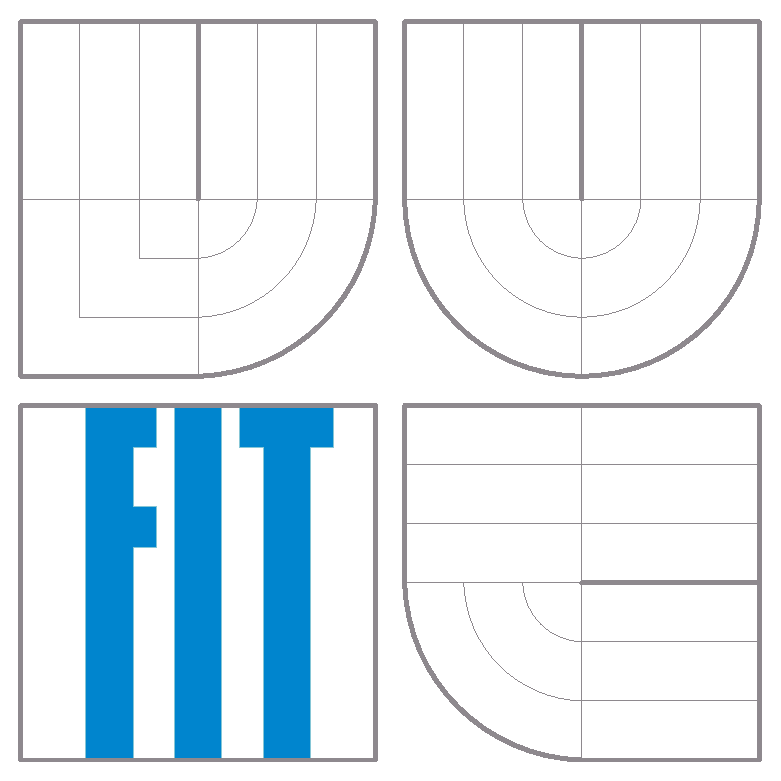
\includegraphics[height=5cm]{images/logo.eps}
	\end{center}
	\vfill
	\begin{center}
		\begin{Large}
			\Course\\
		\end{Large}
		\bigskip
		\begin{Huge}
			\WorkTitle\\
		\end{Huge}
	\end{center}
	\vfill
	\begin{center}
		\begin{large}
			\today
		\end{large}
	\end{center}
	\vfill
	\begin{flushleft}
		\begin{large}
			\begin{tabular}{lll}
				Autor: & \AuthorA, & \url{\AuthorAEmail} \\
				& \AuthorB, & \url{\AuthorBEmail} \\
		
				& & \\
				& \Faculty \\
				& \School \\
			\end{tabular}
		\end{large}
	\end{flushleft}
\end{titlepage}		

\tableofcontents

% ----- obsah -------------------------------------------------------------
\newpage

\section{Zadání}

\begin{itemize}
	\item Implementace Raytraceru pomocí technologie CUDA v~následujícím rozsahu:
	\begin{itemize}
		\item Geometrická primitiva: roviny, koule, trojúhelníky, válce
		\item Načítání modelů z~běžně používaných formátů
		\item Phongův osvětlovací model
		\item Bodové zdroje světla a~stíny
		\item Odlesky
	\end{itemize}
	\item Akcelerace raytracingu na GPU
	\item Vygenerování demonstrační scény a~její vykreslení
	\item Srovnání s~CPU implementací
\end{itemize}

%---------------------------------------------------------------------------
\section{Použité technologie}

Použité technologie:

\begin{itemize}
	\item NVidia CUDA 6.5, C++11
	\item Microsoft Visual Studio 2013 + NVidia NSight
	\item GLUT
\end{itemize}

Je přiložen projekt pro Visual Studio (testováno na Microsoft Visual Studio 2013). Pro samotný překlad je pak třeba mít nainstalované NVidia CUDA 6.5. a~používat překladač podporující C++11.

%---------------------------------------------------------------------------
\section{Výsledky a~použité znalosti}

\subsection{Srovnání CUDA a~Aurelius raytracerů}

Raytracer jsme testovali ve srovnání s~CPU Raytracerem Aurelius, veřejně dostupným Raytracerem pro předmět PGR.

Vzhledem k~tomu, že oba Raytracery jsou implementovány rozdílně, je komplikované vytvořit identické scény, nicméně lze vytvořit scény podobně komplexní.

\subsection{Testovací scéna}

\begin{figure}[ht]
\begin{center}
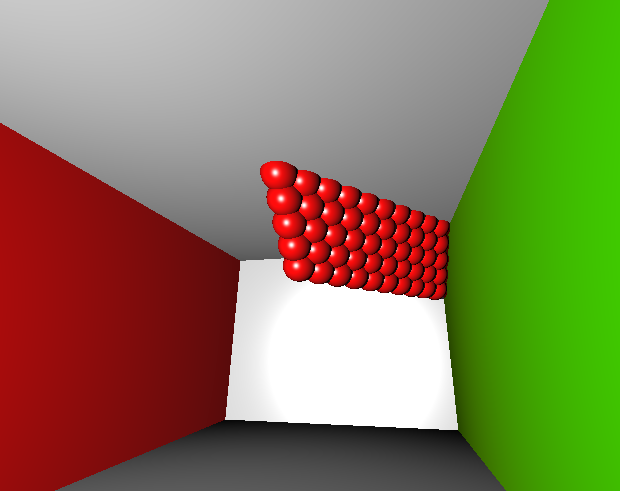
\includegraphics[width=10cm]{images/test-scene.png}
\caption{Testovací scéna na CUDA raytraceru}
\label{fig:theory}
\end{center}
\end{figure}

\begin{itemize}
	\item počet rovin: \textbf{6}
	\item počet koulí: \textbf{5, 10, 20, 50, 100, 500}
	\item hardware: \textbf{NVidia Quadro K1000M, Intel Core i7-3610QM 2.3 GHz}
\end{itemize}

\subsection{Výsledky srovnání}

\begin{table}
\centering
\begin{tabular}{ | l | l | l | l | l | l | l |}
\hline
\textbf{Počet koulí} & 5  & 10  & 20 & 50 & 100 & 500 \\
\hline
\textbf{CUDA} [s] & 0,0193 & 0,0195 & 0,0224 & 0,0341 & 0,05521 & 0,2197 \\
\hline
\textbf{Aurelius} [s] & 0,905 & 1,233 & 1,779 & 3,541 & 6,505 & 30,373 \\
\hline
\end{tabular}
\caption{Srovnání podobně komplexních scén na raytraceru Aurelius a~CUDA raytraceru pro daný počet koulí}
\end{table}

Syntéza raytracerem Aurelius byla cca 100x pomalejší, než-li syntéza podobné scény na GPU. S~komplexností scény roste výpočet Aurelia rychleji.


\begin{figure}[ht]
\begin{center}
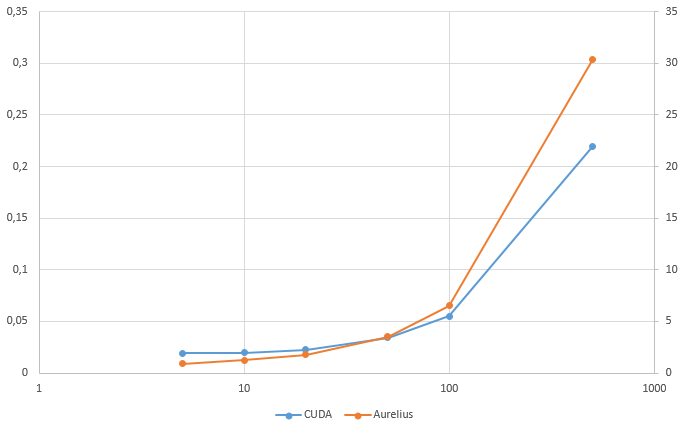
\includegraphics[width=10cm]{images/srovnani.png}
\caption{Srovnání raytraceru Aurelius \textbf{[s]} a~CUDA raytraceru \textbf{[s/100]}}
\end{center}
\end{figure}

\subsection{Paralelizace na GPU}

\subsubsection{Rozvržení paměti} 

Raytracer ke svému běhu potřebuje pouze informace o~scéně:
\begin{itemize}
	\item světla (constant memory)
	\item nastavení kamery (constant memory)
	\item informace o~materiálech (constant memory)
	\item databáze primitiv (constant memory)
\end{itemize}

\paragraph{Světla, nastavení kamery a~materiály} jsou data používaná pro výpočet každého paprsku, je tedy vhodné používat constant memory, která vykazuje nejrychlejší přístupový čas a~zároveň je broadcastována pro všechna vlákna. Diskutabilní je uložení materiálu pro scény, kde jich je hodně. Constant memory je nejen omezena velikostí 64 KB, ale je i~z~důvodu broadcastu neefektivní pro scény, kde paprsky budou trefovat primitiva s~různými materiály.

\paragraph{Databázi primitiv} je vhodné ukládat v~konstantní paměti z~hlediska broadcastu, ale pro scény s~více jak 500-600 primitivy se nevejdeme do max. velikosti constant memory (64 KB), což je i~omezení velikosti scény CUDA raytraceru. Šlo by využít globální paměť, což by však vedlo ke zpomalení.

\subsubsection{Paralelizace výpočtu}

Pro každý pixel syntetizovaného obrazu se vyšle paprsek -- vytvoří vlákno a~to vypočte výslednou barvu (včetně odrazů a~stínů).

\subsection{Optimalizace}

Během implementace jsme tématiku zkoumali a~napadly nás následující optimalizace. Z~časového hlediska, které by často vyžadovaly kompletně přepsat aplikaci a~ve výsledku by nemusely znamenat zlepšení, nejsou z~většiny implementovány.

\subsubsection{Odraz paprsku} 

Při odrazu paprsku od odrazivého materiálu dochází k~vyslání dalšího paprsku. Vlákna, která nic netrefí nebo trefí neodrazivý materiál vracejí výslednou barvu, nicméně stále se musí čekat na vlákna, která se odrážejí. Počítá tak pouze malé množství vláken a~zbytek čeká. 

Nápad na zlepšení je následující:
\begin{enumerate}
	\item Raytracer vyšle paprsek
	\item Zjistí se která vlákna vrátila výsledek (trefila neodrazivý materiál nebo nic) a~která dál chtějí počítat (odrážet se)
	\item Přenese se stav výpočtu zbývajících vláken do paměti
	\item Spustí se kernel pro zbývající vlákna 
\end{enumerate}

\subsection{Akcelerační struktury}

CUDA raytracer využívá jako akcelerační struktury KD-tree a~BVH. Nejedná se sice o~rozšíření implementovaná v~rámci rozsahu předmětu GMU, nicméně i~samotné struktury lze akcelerovat.

Intuitivním přístupem je sestavit struktury na CPU a~následně vše nakopírovat na GPU. Struktury je ale možné sestavit i~na GPU, což je mnohem rychlejší. \cite{karras}



%---------------------------------------------------------------------------
\section{Ovládání vytvořeného programu}

Raytracer nabízí možnost využití některých akceleračních optimalizací avšak pro tyto optimalizace je nutné raytracer znovu přeložit. Volbu provedeme pomocí podmíněného překladu za použití konstant v~souboru constatns.h. Pro BVH je nutné definovat proměnou ACC\_BVH pomocí \#define ACC\_BVH. Pro KD-Tree konstantu ACC\_KD\_TREE. Stejně jako optimalizační algoritmy je možné využít různých aplikací raytraceru (neostré  stíny -- OPT\_SOFT\_SHADOWS, hloubka ostrosti -- OPT\_DEPTH\_OF\_FIELD, automaticky pohyb kamery -- OPT\_CAMERA\_SHIFT nebo bilineární samplování -- OPT\_BILINEAR\_SAMPLING). 

V~raytraceru je možné pomocí kláves Q, W, E, A, S, D nastavit pozici kamery (A~a~D ve směru osy x, W a~S~ve směru osy y, Q a~E ve směru osy z) avšak bod, na který kamera směřuje se nezmění. Pokud je raytracer přeložen pro výpočet hloubky ostrosti je možné měnit ohniskovou vzdálenost pomocí šipky nahoru a~dolů.

%---------------------------------------------------------------------------



\subsection{NVidia CUDA}
Hlavní co jsme museli nastudovat jsou vědomosti ohledně technologie CUDA tedy struktura pamětí, jak je používat pomocí jejího C++ API a~v~kombinaci s~programováním na CPU.

K~debugování a~programování jsme následně využívali vývojové prostředí Microsoft Visual Studio 2013 s~NVidia NSight.

\subsection{Krátce o~Bounding Volume Hierarchy}
Jedná se o~akcelerační strukturu při výpočtech v~počítačové grafické.

\paragraph{Konstrukce}
\begin{itemize}
	\item Určí se konstanta pro počet objektů v~nejnižší vrstvě stromu, tj. kolik listů bude mít každý předposlední uzel stromu.
	\item Řadíme objekty podle svých souřadnic (zda-li X, Y nebo Z~záleží na programátorovi) a~dělíme prostor vždy na 2.
	\item Skončíme ve chvíli, kdy v~daném podprostoru je méně objektů, než-li námi daná konstanta, tyto objekty pak přidáme do seznamu daného uzlu
\end{itemize}

\paragraph{Výhody} V~případě raytracingu nemusíme testovat zda-li paprsek protne všechny primitiva ve scéně, ale vždy testujeme zda-li trefíme některý z~podprostorů: kořen stromu má 2 podprostory, každý z~nich zase další 2. Ve chvíli kdy narazíme na podprostor, který již nemá žádné další, ale pouze jednotlivé listy, tak provedeme test na průnik pouze těch primitiv obsažených pod daným uzlem. Počet testů je tak roven \verb|HLOUBKA STROMU * 2 + POČET LISTŮ NA UZEL|, což bývá podstatně méně u~velkých scén, než-li celkový počet primitiv.


%---------------------------------------------------------------------------
\section{Rozdělení práce v~týmu}

\begin{itemize}
\item \textbf{Jan Bureš}: Phongův osvětlovací model, úprava bilineární interpolace, především raytracing-části raytraceru, hloubka ostrosti, neostré stíny
\item \textbf{Pavel Macenauer}: Základní kostra programu, optimalizace využitých paměťových jednotek, základ pro bilineární interpolaci, především CUDA-části raytraceru 
\end{itemize}

%---------------------------------------------------------------------------
\section{Co bylo nejpracnější}

\begin{itemize}
\item \textbf{Jan Bureš}: Na celé práci bylo asi nejsložitější upravit algoritmus sledování paprsku tak, aby fungoval na architektuře CUDA. Dále pak správné rozdělení vláken do warpů a~rozhodnout, který druh paměti použít pro které proměnné. Mno času bylo zapotřebí také věnovat rekurzi, kterou by sice CUDA měla podporovat od verze 3.0, ovšem stále program havaroval kvůli přetečení zásobníku.
\item \textbf{Pavel Macenauer}: Nejprve celé zprovoznění CUDy a~způsob, kterým předávat data mezi OpenGL, CUDou a~následně je vykreslit stálo mnoho nervů a~několik šálků kávy navíc. Především proto, že nové CUDA 3.0 API obsahuje nové metody pro komunikaci s~OpenGL, nicméně dokumentace a~materiály k~tomu jsou především v~podobě vygenerované dokumentace od společnosti NVidia. Dále ještě za zmínku stojí implementace BVH a~celkové nastudování o~principů.
\end{itemize}
%---------------------------------------------------------------------------
\section{Zkušenosti získané řešením projektu}

Naučili jsme se více o~architektuře CUDA a~získali představu o~psaní paralelních algoritmů, vyzkoušeli si implementovat phongův osvětlovací model a~raytracer v~praxi. Dále jsme si prostudovali možné algoritmické optimalizace raytraceru a~některé z~nich implementovali.


%---------------------------------------------------------------------------
\section{Autoevaluace}

\paragraph{Technický návrh (85\%):} 
Tvorbu programu jsme si naplánovali na jednotlivé iterace, a~tak až na pár úprav, které nás napadli během implementace nebylo nutné přepisovat již implementované části. Především se jednalo o~části týkající se správy paměti, kdy s~každým typem paměti na GPU se pracuje trochu jinak.

\paragraph{Programování (75\%):}
Kód je dobře strukturovaný, ale mohl by být více okomentován, např. pro vygenerování použitelné doxygen dokumentace. 
Implementovaný raytracer je možné dále rozšiřovat a~bez sebevětších komplikací přidávat další doplňky.

\paragraph{Vzhled vytvořeného řešení (80\%):} 
Scéna vypadá celkem pěkně, velmi zřídka lze pozorovat tečky, které narušují plynulost obrazu. Způsobené jsou pravděpodobně používáním datového typu float a~nepřesností, které způsobuje. Některé optimalizace kvalitu obrazu mírně zhorší, ale vždy dle očekávání. Není problém do budoucna do implementovat i~další primitiva, která by umožnila tvorbu komplexnějších scén.

\paragraph{Využití zdrojů (90\%):}
Hodně jsme využili již implementovaný raytracer Aurelius k~lepšímu pochopení raytracingu a~trochu méně pak dostupnou literaturu. Zdroje o~CUDě a~jejím zapojení jsme získali především z~vyhledávače Google.

\paragraph{Hospodaření s~časem (70\%):}
Začali jsme hned jak jsme obdrželi zadání, nicméně chvíli trvalo, než jsme vůbec měli něco co by něco vypočítalo na CUDě a~předalo k~zobrazení. Uprostřed semestru naše snaha mírně opadla kvůli jiným povinnostem ve škole. Na závěr jsme se snažili vše dokončit v~čas, což se i~povedlo.

\paragraph{Spolupráce v~týmu (95\%):}
Od začátku jsme komunikovali ohledně podmínek spolupráce. Následné programování pak probíhalo bez problémů a~o~všem jsem se navzájem informovali přes instantní mluvítka jako Skype nebo Facebook. Veškeré změny jsme pak evidovali v~repositáři na serveru GitHub.com, kde jsme i~vybudovali společné vývojové prostředí.

\paragraph{Celkový dojem (90\%):} 
Celý projekt se nám jevil mírně obtížnější vzhledem k~ostatním projektům na škole, především z~důvodu dostupnosti materiálů, kterých je na internetu spousty, nicméně vyfiltrovat z~nich použitelné informace je časově náročné. 
Získané vědomosti a~zkušenosti jsou určitě přínosem. 
Vybrali jsme si téma projektu kvůli architektuře CUDA, kterou jsme předtím v~praxi nikdy nepoužívali a~tímto jsem si udělali nejen lepší představu o~samotné technologii ale i~o~moderních grafických kartách a~naučili se pracovat s~další technologií, která má své místo v~softwarové budoucnosti. Celý projekt byl zajímavý také tím že jsme si vyzkoušeli vytvořit grafickou aplikaci úplně od začátku.


%---------------------------------------------------------------------------
\section{Doporučení pro budoucí zadávání projektů}

Následující body jsou spíše nápady pro vytvoření možnosti v~daném časovém rozsahu zpracovat komplexnější projekt a~přeskočit onu fundamentální část projektu "aby to něco dělalo":
\begin{itemize}
	\item Specifikovat požadavky k~zadanému tématu (která primitiva implementovat, do jaké míry implementovat raytracer, případně vypsat, co změřit ...)
	\item Sestavit kostru projektu, např. projekt v~MS Visual Studiu/QMake/Makefile s~potřebnými hlavičkovými soubory obsahující prototypy metod
\end{itemize}

%---------------------------------------------------------------------------

\bibliographystyle{plain}

\nocite{pgr-raytracing}
\nocite{aurelius}
\nocite{pgp-optimalizace}
\nocite{cuda-doc}
\nocite{phong-wiki}
\nocite{so-stack}
\nocite{bvh}
\nocite{cmemory}
\nocite{trier}
\nocite{cite1}
\nocite{cite2}
\nocite{cite3}
\nocite{cite4}
\nocite{STRACHOTA}
\nocite{HART}
\nocite{COOK}
\nocite{STOCHASTIC}
\nocite{FUSSELL}



\bibliography{reference}
\addcontentsline{toc}{section}{Literatura}


\end{document}

